\section{Introduction}
\label{sec:intro}

\begin{figure*}[!tbh]
%\centering
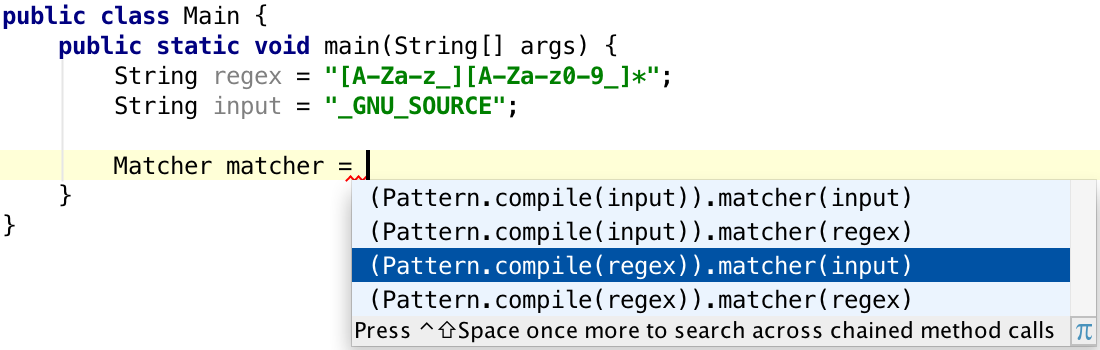
\includegraphics[natwidth=\textwidth]{RegexMatcher.png}
\caption{{\ourTool} suggesting five highest-ranked 
well-typed expressions synthesized from declarations visible at a given program point\label{fig:screenshot1}}
\end{figure*}


Software development provides a high degree of freedom and
many different approaches can be adopted for writing
code. Still, when writing a program, the developer needs to follow
the strict rules determined by the programming language. While coding, the developer often knows the
approximate structure of the desired expressions but still may write code
that does not compile, because some fragments are not well-typed.
Such mistakes occur mainly because the developer does not
know by heart how to choose and properly combine all the necessary
declarations visible from the scope. By the term ``declarations'' 
we refer to all the elements visible in the scope, such as variables, functions, and class
hierarchy declarations. Moreover, modern libraries often evolve into complex 
application programming interfaces (APIs) that provide
a large number of declarations. For this reason 
it is hard, if not impossible, to learn the specifics of
the declarations and their utilization. In a typical scenario when code does not compile, the compiler outputs
an error message with the expression that is at the source of the
error. Still, on many occasions the written expression reflects the
intended structure of the code. 

As an illustration, a programmer might expect the Java code
\begin{lstlisting}
BufferedReader br = new BufferedReader("file.txt");
\end{lstlisting}
to open a file called ``file.txt". However, this code will not compile since \texttt{BufferedReader} accepts only a \texttt{Reader} interface implementation as an argument. After consulting the documentation, the programmer corrects the previous line to
\begin{lstlisting}
BufferedReader br = 
   new BufferedReader(new FileReader("file.txt"));
\end{lstlisting}
Mistakes like these are common when exploring a new API, or a new language, 
since classes are often composed in non-intuitive ways. A survey conducted on 
157 software engineers at Microsoft \cite{LaToza:2006} revealed that
$56\%$ admit to spending a large amount of time trying to understand code that other people wrote, and $41\%$ agree that the amount of example code adapted for a production setting is a serious problem. We believe that the time spent perusing the API documentation could be spent actually writing the application-specific parts of the code. 

In this paper we describe a tool, called \ourTool, which
automatically repairs code expressions based on the hinted structure
of the ill-typed code. \ourTool finds well typed expressions that are as close as 
possible to the given (potentially) ill-typed expression - we call such an
input expression, a {\em backbone} expression. 

Additionally, \ourTool can also be 
seen as a synthesis tool. It extends the functionality described in \cite{MandelinetALL2005Jungloid, GveroETAL13CompleteCompletionTypesWeights, PerelmanGBG12}.
In the light of the program repair, the synthesis aspect of \ourTool can be 
considered as a repair of the empty expression. A user does not need to provide a backbone expression -- it is sufficient to declare a variable of an arbitrary type. Based on that type \ourTool can synthesize corresponding code fragments. The synthesized code has the given type and it can contain user defined 
values, as well as methods from the API. 

Our tool can be applied in interactive scenarios like IDE code completion, to rank expressions 
based on their similarity to ill-typed code. Preferably, the best
suggestions will correct the code keeping its overall structure.
Another application is in providing automated repair in the compilation process.

\ourTool is a tool based on a graph algorithm for synthesizing expressions of a certain type in a programming language. As an algorithm, a synthesis process is further 
extended so that it also repairs ill-typed expressions. We believe that this construction will prove useful a useful tool for synthesis in other contexts, as well.
\ruzica{we need to say more here about the algorithm, talk about costs }



A research on improving the software development process covers a large number of topics such as an automated
program repair
\cite{LeGoues:2012:ROI:2330163.2330296,WeiETAL10AutomatedFixingProgramsContracts,PeiETAL11CodebasedAutomatedProgramFixing},
enhancements of compilation process messages
\cite{Burke87apractical,Hammond198451,Lerner:2007:STM:1250734.1250783}, and
providing assistance to developers through inference of code
\cite{GveroETAL13CompleteCompletionTypesWeights,MandelinetALL2005Jungloid,KneussETAL13SynthesisModuloRecursiveFunctions,KuncakETAL13ExecutingSpecificationsSynthesisConstraintSolvingInvitedTalk,PerelmanGBG12}.
As a result, a vast number of tools was created around a common
high-level goal of facilitating software development.
The manner in which such tools operate can be roughly divided into two
categories: (1) as automated processes within the compiler 
(2) or as development assistants that require a certain level of
interaction, usually through an IDE interface.
Many of the techniques behind these tools such as parsing error recovery by altering the
input \cite{Burke87apractical}, a heuristic search for syntactically
correct terms \cite{PerelmanGBG12}, a modification of
abstract syntax trees and types \cite{Lerner:2007:STM:1250734.1250783}, and an inference
of semantically correct code fragments
\cite{KneussETAL13SynthesisModuloRecursiveFunctions}, share common insights.

Motivated by the advances in both the theory of programming languages and
techniques that are foundations of tools for software development, our
approach addresses the problem of code repair from a new perspective,
by providing an algorithm that extends existing and incorporates new
ideas.  The reason why our tool goes beyond the existing line of
work is three-fold: (1) the algorithm tries to solve more general code
repair problems constrained with the structure of given ill-typed
terms, (2) it focuses on repairing programs in as much accurate way as
possible, according to the given hint and weight heuristics, while
providing useful theoretical guarantees about the utilized repair
algorithms, (3) it is fitting for realization as both an interactive
and automated software development tool.

\ruzica{clearly this part has to be written once the paper is finished}
The contributions of this paper are:
\begin{itemize}
	\item We formulate the problem of repairing ill-typed expressions.
	As input to the problem we take a backbone expression and 
	the set of repair declarations. We introduce weak long normal 
	form that allows a systematic search and a construction of the well-typed expressions.
	We identify special symbols used to extend the expressiveness of the input.
	\item We propose a novel repair calculus that specifies the rules that
	we use to derive a well-typed term from a backbone expression.
	The calculus describes how to fix a term using declarations with multiple arguments.
	\item We propose an algorithm that finds the best well-typed expression based on 
	weights system introduced in \cite{GveroETAL13CompleteCompletionTypesWeights}.
    We show that the algorithm is polynomial given a certain class of ill-typed expressions.
    \item We present a sound and complete algorithm that takes the ill-typed expression and 
    finds a set of best solutions. The algorithm is based on A* search.
\end{itemize}


